\section{Implementacija}
Implementacija se sastoji od dva dijela. Prvi dio opisuje igru Texas Hold'em poker te izradu igre u python programskom jeziku, a drugi dio se odnosi na izradu agenta koji treba naučiti igrati ovu igru i biti uspješan na jednoj osnovnoj razini.
\subsection{Implementacija igre}

\subsubsection{Poker}
Jako poznata igra karata, nastala u Americi, čiji korijeni dosežu od perzijske igre As-Nas. 
Kroz 19. stoljeće igra se razvijala s raznim dodacima i varijacijama.
Postaje jako popularna kroz 20. stoljeće kada su se počeli održavati turniri. Ta popularnost se proširila svijetom uz igranje i održavanje turnira putem interneta, te turnira koji snimaju 
karte svih igrača tako da gledatelji mogu bolje pratiti igru. 

Iako postoje razne verzije pokera, svi dijele jednaka osnovna pravila igre. Igra se sastoji od 52 igrajuće karte, koje se mogu vidjeti na slici~\ref{fig:poker_cards}, od kojih se 13 karata 4 puta ponavljaju samo s različitim simbolima. 
Vrijednosti tih 13 karata su: brojevi od 2 do 10, dečko, kraljica, kralj i as. Cilj svakog igrača je sebi složiti najjaču ruku kombinacijom od pet karata.
\\[\intextsep]
\begin{minipage}{\linewidth}
	\centering%
	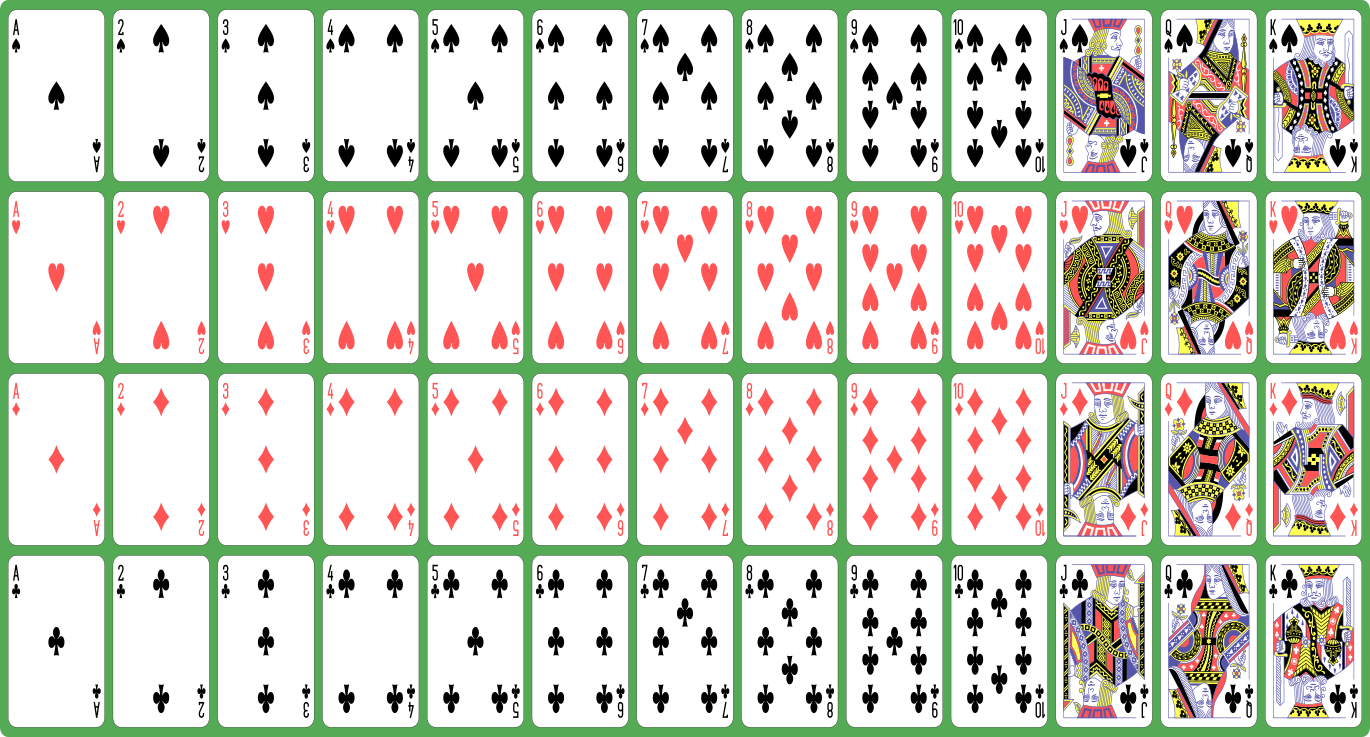
\includegraphics[width=0.8\linewidth,clip=]{images/poker_playing_cards.png}%
	\figcaption{Izgled igračih karata za poker}%
	\label{fig:poker_cards}%
\end{minipage}
\\[\intextsep]

Ruke poredane od najslabije do najjače:
\begin{itemize}
	\item Visoka karta (eng. \textit{high card}): Igrač nije uspio složiti odgovarajuće kombinacije i gleda se karta s najjačom vrijednosti. Karte poredane po jačini (od najslabije prema najjače):
	brojevi od 2 do 10 (veći broj znači snažnija karta), dečko, kraljica, kralj pa as.
	
	\item Par (eng. \textit{pair}): Igrač je od bilo koje vrijednosti uspio skupiti dvije iste karte.
	\item Dva para (eng. \textit{two pairs}): Ruka se sastoji od dvije karte s jednom vrijednosti i dvije s drugom.
	\item Tris (eng. \textit{tris}): Bilo koja vrijednost karte 3 puta.
	\item Skala (eng. \textit{straight}): Pet različitih vrijednosti poredanih tako da je svaka sljedeća karta za jednu vrijednost jača od prethodne.
	
	\item Boja (eng. \textit{flush}): Pet karata istog simbola.
	\item Puna kuća (eng. \textit{full house}): Tri karte iste vrijednosti i dvije druge karte istih vrijednosti.
	\item Poker (eng. \textit{poker}): Četiri karte istih vrijednosti.
	\item Skala u boji (eng. \textit{straight flush}): Pet vrijednosti gdje je svaka sljedeća za jednu vrijednost jača od prethodne i sve u istim simbolima.
	
	\item Kraljevska skala u boji (eng. \textit{royal flush}): 10, dečko, kraljica, kralj, as u istim simbolima.
\end{itemize}

\subsubsection{Pravila igre}
Igra koja se implementirala se naziva \emph{Limit Texas Hold'em turnir}, i pravila su sljedeća. 
Potrebno je bar dva igrača, tri da bude zanimljivo pa do nekih desetak (nema neke fiksne gornje granice, 
ali najčešće je deset). Prije početka igre svi igrači uplaćuju dogovoreni iznos novca za sudjelovanje u igri, te dobiju za uzvrat žetone vrijednosti uloženog novca. Igrači sjede za ovalnim stolom i jednoga od igrača se određuje kao djelitelja. Djelitelj dobije poseban žeton koji ga vidljivo označava kao takvog. Karte se izmiješaju i svakom igraču se dodjele dvije karte, u smjeru kazaljke na satu. Ove dvije karte su za ostale igrače tajna, znači svaki igrač nastoji da jedini vidi te karte, zapamti ih i po mogućnosti do kraja kruga ih drži okrenute naopako na stolu. U prvoj fazi \emph{pre flop} nakon dijeljenja karata prvi igrač lijevo od djelitelja je prisiljen uložiti žetone u visini pola vrijednosti minimalnog uloga, taj ulog se naziva \emph{small blind}, a sljedeći ulaže \emph{big blind} cjelokupan minimalni ulog, također prisiljeno. Prisiljeni ulozi služe kako bi u svakom krugu postojala neka dobit, a i da skrati igru koja i onako zna potrajati satima. Ostali igrači nakon njih imaju mogućnost birati hoće pratiti (eng. \textit{call}), što znači da moraju sve skupa uložiti koliki je trenutačni najveći ulog, hoće li odustati i preklopiti karte (eng. \textit{fold}), gdje odbacuju karte iz ruku i isključeni su iz igre do kraja kruga ili će povisiti (eng. \textit{raise}) ulog, u kojem slučaju trenutačni ulog postane jednak prošlom plus minimalni iznos za ulaganje. U trenutku kada su ostali igrači napravili potez, prvi igrač do djelitelja mora nadoplatiti ostali iznos za pratiti ili izabrati neki od drugih poteza i na kraju igrač koji je morao prisilno uložiti minimalni ulog ima mogućnost napraviti potez, s tim da ako nije bilo povećavanja uloga umjesto da prati (eng. \textit{call}) ima potez potvrde (eng. \textit{check}), što znači da nema namjeru povisiti ulog niti izostati iz trenutačnog kruga. Kada svi igrači potvrde potez djelitelj izbacuje jednu kartu iz igre, i kaže se da se karta izgori (eng. \textit{burn}), te na sred stola okrene 3 karte vidljive svima, to je \emph{flop} faza. 
Karte okrenute na srid stola su karte zajednice (eng. \textit{community cards}) i svaki igrač ima pravo svoju ruku od pet karata složiti s bilo kakvom kombinacijom svoje vlastite ruke i karata zajednice. Slijedi potez svakog igrača, međutim u ostalim fazama nema prisilnog ulaganja. U \emph{turn} fazi djelitelj opet izbacuje kartu i okrene sljedeću na stol, ponovno svi igrači određuju svoj potez. \emph{River} faza je identična \emph{turn} fazi, tako da na kraju su pet karata okrenute na sredini stola i bar dva igrača u igri. Sada igrači okreću karte i izjasne se koju kombinaciju su sebi složili, i igrač s najjačom kombinacijom kupi ukupan ulog (eng. \textit{pot}), ili ako imaju nekoliko igrača istu jačinu onda ga dijele. Ako se u bilo kojoj fazi dogodi da svi osim jednog igrača odustaju, preskaču se ostale faze i igrač skuplja ukupni ulog. Postoji još i poseban potez ulaganja svega (eng. \textit{all in}) gdje igrač kada nema dovoljno žetona za uložiti, ulaže sve što ima i u slučaju gubitka izbačen je iz igre. Dobitnik je igrač koji zadnji ostaje u igri i nagrada mu je ukupan uplaćeni ulog svih igrača. Pošto je igra nepotpuno informirana igra postoji mogućnost blefiranja gdje igrač s lošom rukom ulaže i/ili diže ulog da stvori dojam da ima jaku ruku na račun koje će neki ili svi ostali igrači odustati u trenutačnom krugu.


\emph{Limit} označava da je svaki ulog fiksan i u svakoj fazi su dozvoljena tri ponovna povisivanja uloga (eng. \textit{reraise}), gdje za razliku od \emph{no limit} igrač može povisiti najmanje minimalan ulog a najviše koliko hoće te nema ograničen broj ponovnog povisivanja uloga.

\emph{Texas Hold'em} je način igre s dvije tajne karte i pet javnih, dok u klasičnom pokeru svaki igrač dobije pet karata (koje su drugim igračima tajna) te ima pravo izbaciti nijednu, nekoliko ili sve karte i onoliko koliko izbaci dobije novih, te na kraju to postaje konačna ruka.

\emph{Turnir} podrazumijeva da svi igrači na početku uplate jednak iznos i igra se dok svi ispadnu osim jednog, dok u \emph{cash game} može igrač ponovno kupiti žetone za nastaviti igrati, može odustati od igre 
iako nije izgubio sve žetone te ih unovčiti, a mogu čak naknadno doći i novi igrači.

\subsubsection{Program}
Pisane su klase koje predstavljaju karte i špil. Klasa \pythoninline{Card}, koja je dana u ispisu~\ref{poker_card}, predstavlja jednu kartu koja ima 3 vrijednosti: oznaku, symbol i vrijednost. Dok klasa \pythoninline{Deck}, koja je dana u ispisu~\ref{poker_deck} stvara špil od 52 odgovarajuće karte za poker te implementira metode za miješanje, dijeljenje i izbacivanje karata.

\pythonexternal[caption={Klasa karta}, label=poker_card]{code/poker_card.py}
\pythonexternal[caption={Klasa špil}, label=poker_deck]{code/poker_deck.py}

Svi igrači koji žele sudjelovati u poker turniru moraju biti naslijeđeni od apstraktne bazne klase. \pythoninline{Player} koja je prikazana u ispisu~\ref{poker_base_player}. 

\pythonexternal[caption={Bazna klasa igrač}, label=poker_base_player]{code/player.py}

Bazna klasa prima količinu žetona kao parametar u konstruktor, implementira osnovne operacije svakog igrača, koje su: primanje žetona, trošenje žetona, primanje karata, pokazivanje ruke, uništavanje ruke i prikaz vrijednosti žetona. Bazna klasa definira apstraktnu metodu \pythoninline{make_move} za odrađivanje akcije koja prima trenutačno stanje igre te niz mogućih, odnosno, dozvoljenih akcija. Trebala bi vratiti jednu od akcija koja se nalazi u nizu dozvoljenih. U suštini bi trebao inteligentni agent na osnovu određenog stanja u igri donijeti odluku o najboljem sljedećem potezu. Ostavlja se fleksibilnost za buduće pokuse gdje se na osnovu broja informacija o okruženju, odnosno, stanja u igri, mjeri kvaliteta odluke agenta o sljedećem koraku (agent se smatra inteligentnijim kad sa što manje informacija donese dobru odluku). 

\iffalse
Klasa \pythoninline{Table} u konstruktor prima niz klasa \pythoninline{Player} i u konstruktoru inicijalizira objekt za svakog igrača. Koristi vlastitu implementaciju igrača, koja je kao pomoćna klasa za radom s igračima za stolom. 
\fi
%\pythonexternal[caption={Pomoćna klasa igrači za stolom}, label=poker_table_players]{code/table_players.py}

Glavni dio cijele igre je klasa \pythoninline{Table}, brine se o rasporedu igre te primjenjuje pravila u Limit Texas Hold'em turniru. Prima niz klasa kao ulazni parametar u konstruktor. Provjerava da li su sve klase naslijeđene od bazne klase igrača, inicijalizira sve igrače s proslijeđenim klasama, dodjeljuje im žetone i pokreće igru. Stol posjeduje vlastitu klasu igrača koja enkapsulira baznu klasu, te dodatne podatke koji služe za praćenje same igre. Ova pomoćna klasa prikazana je ispisom~\ref{poker_table_players} u dodatku. Nakon što stol rasporedi igrače, započinje s turnirom, prolazi kroz sve faze igre dok ne ostane samo jedan igrač. Prati ulaganja svih igrača, i na kraju dijeli ukupni ulog odgovarajućim igračima. Klasa za igrače za stolom smještena je u datotečnom sustavu unutar direktorija za stol. Namjena je usko vezana za igru tako da njen domet ne bi smio prelaziti sami stol. Kvalitetan software bi se trebao sastojati od neovisnih elemenata, što omogućuje jednostavnije testiranje svakog elementa te razmjenu ili dodavanje novih elemenata. Iako se dosta toga u ovoj klasi razdvojilo (kao npr. izrađena je odvojena klasa koja određuje jačinu krajnje ruke), i dalje ima prostora za refaktoriranje. Tu bi sljedeći korak bio izbaciti podjelu žetona na kraju svakog kruga u zasebnu klasu i tako rasteretiti klasu stola. Najkompleksnija funkcija cijele igre je na kraju svakog kruga koja dijeli žetone dobitnicima. Pošto mora pokriti sve mogućnosti, dosta problematično postaje kada je to nekom ili nekoliko igrača posljednji potez \emph{all in}, tada nastaje nekoliko razina dobitnika te se svakom dobitniku mora izračunati točan dobitak. Postoje slučajevi gdje nakon dijeljenja \emph{pota} ostaju žetoni jer ih nije moguće podijeliti na broj dobitnika. U tom slučaju svaka kuća ima svoja pravila i većinom se igra po nekom dogovoru za taj slučaj. Ovdje se taj ostatak prenese u sljedeći krug, igra se normalno i na kraju dobitnik tog kruga, ili dobitnici ako je moguće među njima podijeliti bez ostatka, pokupe ostatak od prethodnog kruga. Kroz izradu igre, klasa \pythoninline{Table} je poprimila preveliku odgovornost i previše stvari se odvijaju u toj klasi, te se kroz refaktoriranje izdvojilo klasu koja računa jačinu ruke. Bodovni sustav je osmišljen tako da najjača ruka nekog tipa ruke ima manje bodova od najslabije ruke jačeg tipa. U dodatku se nalazi klasa koja pronalazi konačnu ruku i dana je u ispisu~\ref{poker_strongest_final_hand_finder}. Koeficijent svake vrste ruke dan je ispisom~\ref{poker_final_hand_type}.

\pythonexternal[caption={Koeficijenti vrste ruke}, label=poker_final_hand_type]{code/final_hand_type.py}

Vrijedi još spomenuti prikaz informacija o igri, gdje se implementirao uzorak dizajna promatrača (eng. \textit{observer design pattern}) isto poznat kao objava i preplata (eng. \textit{publish and subscribe}). Koristi se najčešće kada više elemenata zahtijevaju iste informacije te promjene tih informacija, kao npr. za prikaz na drugačiji način. Efektivno razdvaja logiku izvršavanja i prikaz informacija. Sastoji se od dvije komponente, od objavitelja koji drži sve pretplatitelje i samog pretplatitelja. Objavitelj omogućuje dodavanje i odstranjivanje pretplatitelja te obavještava pretplatitelje o promjenama. Svaki pretplatitelj sam za sebe definira na koji način će koristiti informacije i kako se promjene izražavaju. Implementacija objavitelja u Python k\^odu prikazana je ispisom~\ref{poker_publisher}. S time se oslobodila klasa \pythoninline{Table} da se brine o bilo kakvom načinu za prikaz informacije o stanju igre, samo mora definirati metode koje dodaju i odstranjivaju pretplatitelje i u određene trenutke pozvati \pythoninline{notify} funkciju od objavitelja.

\pythonexternal[caption={Objavitelj}, label=poker_publisher]{code/publisher.py}

Implementirala su se dva pretplatitelja, jedan koji ispisuje stanje u terminal a drugi koji zapisuje stanje u tekstualnu datoteku. U buduće bi se mogao dodati neki grafički prikaz stanja što ovaj uzorak dizajna omogućuje bez da se mijenja postojeći k\^od, samo se dodaje nova klasa koja nasljeđuje \pythoninline{BaseSubscriber}.

Za osiguranje sigurnosti k\^oda pisani su testovi, te u slučaju izmjene ili dodatka novih funkcionalnosti, prikazuju da li su izmjene utjecale negativno na postojeći k\^od. Postoji disciplina razvoj upravljan testovima (eng. \textit{test driven development}), u kojemu nije dozvoljeno pisati niti jednu liniju produkcijskog k\^oda prije nego je napisan test koji ne prolazi i ne piše se niti jedna linija testnog k\^oda dok postoji test koji ne prolazi. Nakon što postoji test koji ne prolazi piše se produkcijski k\^od koji omogućuje prolaznost testa i vraća se pisanje novog testa. Nažalost ova disciplina nije primijenjena u ovom projektu, iz razloga, što je potrebno, kao u bilo kojoj disciplini, bar nekoliko mjeseci iskustva kako bi se efektivno primijenila. Bez obzira nije se izostavila važnost testova, pa su se za najvažnije funkcije implementirali testovi, iz jednog razloga za provjeru da li k\^od radi u redu i iz drugog, da se za sve buduće promjene može provjeriti ispravnost. Testovi su poslužili u nekoliko trenutaka a pogotovo u fazi refaktoriranja k\^oda. Za testiranje jedinica (eng: \textit{unit test}) koristio se Pythonov modul \pythoninline{unittest} iz razloga jer se nalazi u Pythonovoj standardnoj biblioteci, nije potrebna nikakva instalacija i može se direktno koristiti. Kreiran je direktorij test, te po konvenciji se osigurava da ime svake skripte testa započinje sa \pythoninline{test_}. Svaka klasa koja testira neku jedinicu mora biti naslijeđena od \pythoninline{unittest.TestCase}, i ime svake funkcije koja testira jedinicu također započinje sa \pythoninline{test_}. \pythoninline{TestCase} klasa ima implementirane funkcije za provjeru kao što su \pythoninline{assertEqual}, \pythoninline{assertTrue}, \pythoninline{assertFalse}, ..., također implementiranu funkciju \pythoninline{setUp} koja se izvršava prije svake testne funkcije. U toj funkciji se pripremaju objekt/i za testiranje kako se ne bi trebalo u svakoj funkciji ponavljati iste postupke. Iako se testne funkcije nalaze u istoj klasi objekti kreirani u \pythoninline{setUp} funkciji se ne dijele među testnim funkcijama nego se za svaku funkciju kreira novi. Funkcija \pythoninline{setUp} se eksplicitno ne poziva nego sve to obavlja bazna klasa \pythoninline{TestCase} u pozadini. U dodatku se može promatrati potpuni primjer jednog testa koji je dan u ispisu~\ref{python_test_case}. Osnovna pravila kojih bi se trebali svi testovi držati su da kao prvo moraju biti brzi, u izvršavanju i prikazivanju rezultata. Testovi kojima treba puno vremena se ne izvršavaju često i kao posljedica pojavljivaju se greške u k\^odu. Moraju biti neovisni jedni o drugima, znači ne smije niti jedan test postojati koji se ne može pokrenuti prije nego se pokrene neki drugi test. U bilo kojemu trenutku bi trebala postojati mogućnost pokrenuti bilo koji test u bilo kojem redoslijedu. Trebali bi se moći pokrenuti u bilo kakvom okruženju. Dodatno svi testovi moraju samostalno prikazati da li je test prošao ili ne i koji nije prošao. Test ne smije nikakvu informaciju izbaciti gdje je potrebna ljudska evaluacija rezultata.

\subsubsection{Protivnici}
Za dokazivanje da inteligentni agent napreduje i zna igrati igru, potrebno je modelirati nekog protivnika na osnovu čega se mogu donijeti ovi zaključci. Najosnovniji protivnik s čime se mjeri agent u bilo kojem području strojnog učenja jest agent koji donosi nasumične odluke. U slučaju pokera agent prima dozvoljene akcije u nekom stanju te nasumično izabere jednu od njih. Specifično za poker je ovo previše loš protivnik, jer se u bilo kojemu stanju među dozvoljenim akcijama nalazi \textit{fold}. Jako su rijetke situacije kada igrač odustane od trenutačnog kruga a da nije nitko povisio ulog. Dodatno potpuno nasumičnim biranjem akcija se češće prekida krug, jer su svi igrači osim jednoga odustali, što znači da agent rijetko posjećuje posljedno stanje kruga u kojemu se ocjenjuju ruke. Iz ovog razloga je osnovni protivnik, protiv kojega se inteligentni agent mora iskazati, polu nasumični. Polu nasumični protivnik će slučajnim odabirom izabrati akciju \textit{fold} samo u slučaju kada se povisio ulog. Dodatno se implementirao algoritam s nekom heuristikom. Početnu ruku u \textit{preflop} fazi kada još nema karata na stolu se boduje na osnovu tablice koju su složili David Skalinsky and Mason Malmuth~\cite{starting_hand_groups}. Tablica grupira sve početne ruke u razini od najjače prema najslabijoj. U ostalim fazama se računa jačina ruke metodama koje se naslanjaju na rad: Opponent modeling in poker~\cite{EHS}. U radu se opisuje izračun učinkovite jačine ruke (eng. \textit{effective hand strength}) koja je dana formulom~\ref{eq:ehs}.

\begin{equation}\label{eq:ehs}
EHS = HS \cdot (1 - NPOT) + (1 - HS) \cdot PPOT
\end{equation}

Gdje je $HS$ trenutačna jačina ruke, ne uzimajući u obzir poboljšanje ili pogoršanje buduće ruke. $NPOT$ je negativni potencijal koji uzima u obzir pogoršanje buduće ruke a $PPOT$ pozitivni potencijal koji zadrži poboljšanje buduće ruke. Potpuna implementacija ove formule je računalno jako zahtjevna. Za izračun trenutačne jačine ruke potrebno je generirati sve moguće protivničkove karte u ruci te usporediti jačinu sa svojom rukom, što je još prihvatljivo. Međutim za izračun pozitivnog i negativnog potencijala potrebno je generirati za svaku sljedeću fazu sve moguće karte koje se mogu okrenuti na stolu i usporediti sve moguće protivnikove ruke sa svojom. Pa se iz tog razloga odlučilo koristiti samo trenutačnu jačinu ruke.

\subsection{Implementacija agenta}
Agent se implementirao pomoću PyTorch radnog okvira. Definirani hiperparametri su globalni za cijelu klasu, za brzo i jednostavno mijenjanje. U konstruktoru se provjerava da li postoji Cuda sposobna grafička procesorska jedinica i pohranjuje tu informaciju na sljedeći način \pythoninline{self._device = 'cuda' if torch.cuda.is_available() else 'cpu'}. Stvaranje same umjetne neuronske mreže dano je ispisom~\ref{simple_dqn_create_network}, gdje se može primijetiti kako na osnovu varijable \pythoninline{self._device} sadržaj neuronske mreže pohranjuje u odgovarajućoj radnoj memoriji. Kako grafička procesorska jedinica ima svoju vlastitu radnu memoriju potrebno je u njoj inicijalizirati neuronsku mrežu u slučaju da je se želi koristiti za treniranje.

\pythonexternal[caption={Stvaranje neuronske mreže za DQN}, label=simple_dqn_create_network]{code/simple_dqn_create_network.py}

Neuronska mreža je jako jednostavna, ima samo dva skrivena potpuno povezana sloja s ispravljenom linearnom jedinicom (eng. \textit{rectified linear unit}) kao aktivaciju. Ova aktivacija svaki element koji je negativan postavlja na nulu, a pozitivne ne dira. Sastavljena neuronska mreža se pohranjuje u varijablu \pythoninline{self._policy_net}. Kroz trening se neuronska mreža ažurira na kraju svakog kruga, što znači da se svi potezi do tada moraju na neki način pamtiti. Ovaj način se pokazao da ubrzaje treniranje. Osim poteza se pamti i cjelokupno iskustvo u određenom stanju koje se sastoji od prethodnog stanja, prethodne akcije, prethodne moguće akcije i sljedećeg stanja. Funkcija koja ažurira neuronsku mrežu prikazana je u ispisu~\ref{simple_dqn_update_network}.

\pythonexternal[caption={Ažuriranje neuronske mreže za DQN}, label=simple_dqn_update_network]{code/simple_dqn_update_network.py}

Nagrada koja se prosljeđuje je razlika žetona prije početka kruga i nakon, tako da ako je razlika pozitivna znači da je agent pobijedio, a ako je negativna onda je izgubio. Prije nego se počmu ažurirati vrijednosti u mreži potrebno je pozvati \pythoninline{self._policy_net.train()} funkciju iz PyTorch biblioteke, koja priprema neuronsku mrežu za treniranje. Kod ažuriranje neuronske mreže prvo raspakira iskustvo, potom funkcija \pythoninline{torch.cat} spaja sve elemente u nizu u jedan tensor, jer se to očekuje kao ulaz pozivanjem neuronske mreže. U ovom koraku se dohvaćaju sve q-vrijednosti za prethodno stanje tako da se poziva neuronska mreža s prethodnim stanjem, što se u slučaju običnog q-učenja s tablicom jednostavno radilo indeksiranjem u određeni redak. Sljedeća funkcija \pythoninline{_generate_target_preds} stvara novo izračunate q-vrijednosti za akcije koje se ažuriraju, a to su akcije koje su izabrane u tom stanju. Ostale akcije se ne mijenjaju, što je usporedivo kod običnog q-učenja gdje se ažurira samo jedna ćelija u tablici. Stvaranje ažurirane q-vrijednosti dano je u ispisu~\ref{simple_dqn_generate_target_preds}. Gubitak se računa pomoću funkcije srednje kvadratne pogreške, koja pruža PyTorch \pythoninline{torch.nn.MSELoss()}, na osnovu čega se u povratnoj propagaciji ažuriraju parametri u mreži. PyTorchev \pythoninline{torch.optim} sadrži klase koje su zadužene za ažuriranje neuronske mreže, a u ovom slučaju se koristio \pythoninline{torch.optim.Adam}. Sama inicijalizacija optimizatora se izvršila u konstruktoru klase naredbom \pythoninline{self._optim = optim.Adam(self._policy_net.parameters(), self._alpha)}. U konstruktoru optimizatora se prosljeđuju parametri mreže te stopa učenja. Prije pozivanja funkcije povratne propagacije potrebno je postaviti gradijente na nulu, kako se ne bi zbrajali s prethodno izračunatim, s funkcijom \pythoninline{zero_grad} od optimizatora. Funkcija \pythoninline{loss_backward} računa nove gradijente, a ažuriranje parametara se odvija u \pythoninline{self._optim.step()} ovisno o gradijentima. Na osnovu gradijenta, optimizator povećava ili smanjuje parametar a na osnovi stope učenja, koja je proslijeđena u konstruktor, se određuje količina smanjivanja ili povećavanja. Ovdje se može primijetiti kako PyTorch implicitno manipulira sa svojim grafom o neuronskoj mreži kojeg čuva u pozadini, također koliko pojednostavljuje rad s neuronskim mrežama.

\pythonexternal[caption={Stvaranje ažurirane q-vrijednosti}, label=simple_dqn_generate_target_preds]{code/simple_dqn_generate_target_preds.py}

Unutar funkcije koja stvara q-vrijednosti prema kojima se uspoređivaju trenutno koja mreža izbacuje, događa se nešto neobično. Obično se neuronske mreže treniraju tako da se proslijedi nešto, a onda uspoređuje rezultat s očekivanim i na osnovu rezultata se parametri u neuronskoj mreži ažuriraju. No u ovom slučaju po drugi put se šalje neko stanje u mrežu. Međutim nužno je zadovoljiti Bellmanovu jednadžbu optimalnosti zbog potrebe za $\max_{a'}q_*(s', a')$. U usporedbi s izračunom q-vrijednosti u klasičnom q-učenju, fali dobar dio jednadžbe. Razlog tome je što dio jednadžbe obavlja funkcija gubitka a dio optimizator koji drži stopu učenja.

Izradila se klasa koja prevodi stanje igre u stanje koje je prihvatljivo za agenta. Stanje se prevodilo u jedno vruće k\^odiranje (eng. \textit{one hot encoding}), što znači da se na kraju dobije niz od nula i jedinica.  Minimalni prostor stanja koji je izgledao prihvatljiv je od 83 elemenata, od kojih 52 elementa predstavljaju svaku kartu, gdje su jedinice poznate karte, bez obzira da li se nalaze na stolu ili u ruci. Sljedećih 30 elemenata su ukupan broj žetona, znači da se turnir ograničio na 3 igrača gdje svaki na početku posjeduje 10 žetona. Još se na kraju dodao jedan element koji se odnosi na mogućnost povećanja uloga, kako u Limit Texas Hold'em postoji mogućnost samo tri puta ponovno povećati ulog u svakom krugu.

\subsection{Učenje}
Klasa \pythoninline{SimpleDqnBot}, koja predstavlja agenta, sadrži globalne varijable koje drže hiperparametre treninga. To su alfa (stopa učenja), gamma (stopa popusta buduće nagrade), epsilon (stopa pohlepe) te oznaku da li epsilon propada tijekom treninga. Za učenje proširila se klasa \pythoninline{Table} s mogućnosti pokretanja turnira ispočetka s istim igračima. Sadrži metode koje postavljaju sve objekte u početni položaj s kojim se započinje turnir. Napisana je skripta u kojoj se određuju parametri treniranja, od kojih je najbitnija broj epizoda u kojima se odvija trening. Skripta inicijalizira turnir s agentom q-duboke mreže i dva polu nasumična. Nakon svake epizode pokreće novi turnir i na kraju treninga ispisuje informacije o treningu. Dodatno se na kraju treninga pohranjuje stanje neuronske mreže na tvrdi disk pomoću funkcije \pythoninline{torch.save(self._policy_net.state_dict(), file_name)}. Poslije se može stanje mreže pomoću \pythoninline{self._policy_net.load_state_dict(torch.load(file_path))} ponovno učitati u mrežu. 

\subsection{Rezultati}
Graf nagrade je prikazan kao kumulativni zbroj dobivenih, odnosno izgubljenih, žetona. Mijenjanje raznih hiperparametara je dovelo do raznih rezultata koji se prikazuju u Tensorboardu i vidljivi su na slici~\ref{fig:tensorboard_results}, također su se rezultati prenijeli na tensorboard.dev koje se nalaze na \url{https://tensorboard.dev/experiment/yCxUmVc1TQeV03tQgJCD1g/}. 
\\[\intextsep]
\begin{minipage}{\linewidth}
	\centering%
	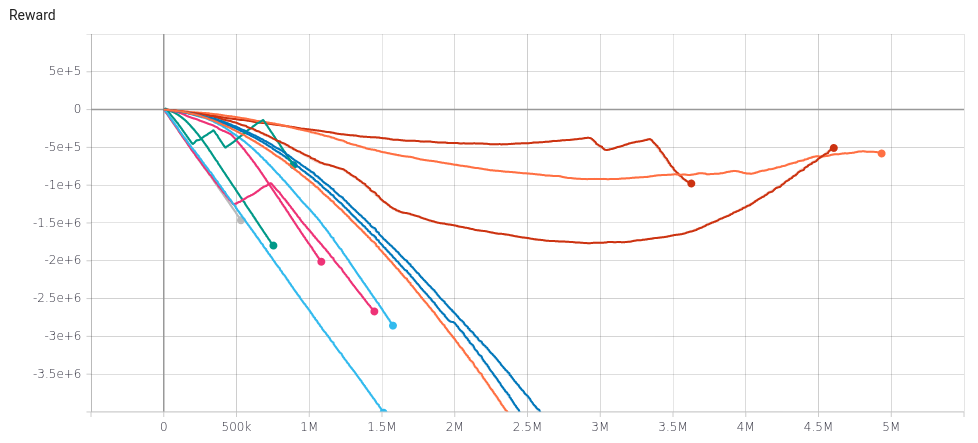
\includegraphics[width=0.8\linewidth,clip=]{images/tensorboard_results.png}%
	\figcaption{Rezultati učenja}%
	\label{fig:tensorboard_results}%
\end{minipage}
\\[\intextsep]

Od svih rezultata bi se moglo odvojiti jednog agenta kojemu je vidljivo da mu se nagrada, nakon nekog vremena, stalno poboljšava. Taj jedan agent na kraju treninga, koji se vrtio u periodu od milijun epizoda, posjeduje najvišu nagradu. Kada bi se tom agentu napredak prikazao kao razlika kumulativne nagrade, njegov graf bi izgledao kao na slici~\ref{fig:agent_nice_graph}. Hiperparametri tog agenta su $10^{-4}$ za stopu učenja, $0.999$ za stopu popusta buduće nagrade te $10^{-6}$ za propadanje stope istraživanja u svakoj epizodi do $0.1$ tijekom treninga. 
\\[\intextsep]
\begin{minipage}{\linewidth}
	\centering%
	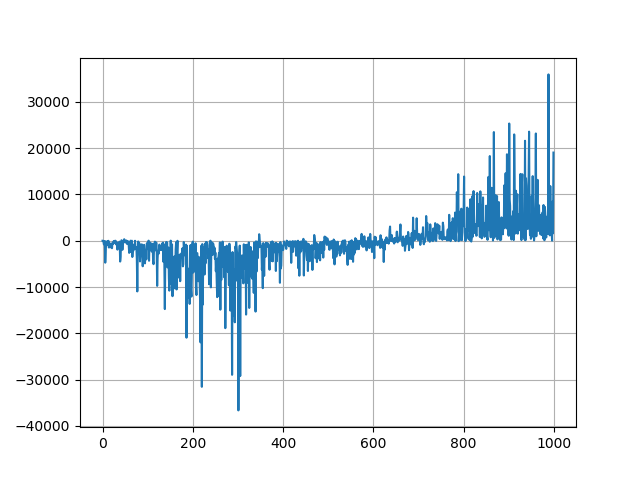
\includegraphics[width=0.8\linewidth,clip=]{images/tensorboard_results_diff.png}%
	\figcaption{Napredak kao razlika nagrade}%
	\label{fig:agent_nice_graph}%
\end{minipage}
\\[\intextsep]
U igri protiv dva agenta neuronska mreža jako loše igra prije treninga, međutim nakon milijun epizoda treninga agent s neuronskom mrežom je u stanju pobijediti u skoro 60\% slučajeva, što je prikazano slikom~\ref{fig:agent_results}.
\\[\intextsep]
\begin{minipage}{\linewidth}
	\centering%
	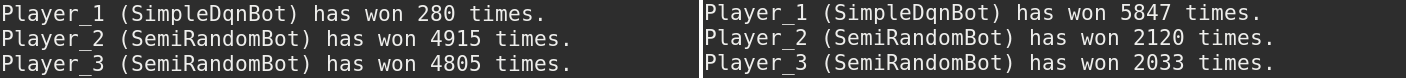
\includegraphics[width=0.8\linewidth,clip=]{images/training_results_0.png}%
	\figcaption{Usporedba agenta prije i poslije treninga}%
	\label{fig:agent_results}%
\end{minipage}
\\[\intextsep]

\subsection{Napredak}
Nadalje su se pokretali pokusi napredovanja mreže, tako da agent uči igrajući protiv protivnika koji donose odluke o sljedećoj akciji na osnovi jačine trenutne ruke. Svi pokusi sa različitim hiperparametrima su bili neuspješni. Detaljnim uvidom u izbor akcije nakon treniranja, primjetilo se da neuronska mreža pretežito izabere akciju \textit{fold}. Znači mreža nije uspješno naučila igrati igru, te je zaključila da sa akcijom \textit{fold} najduže ostaje u igri. Iz tog razloga se odlučilo promijeniti algoritam učenja. U algoritam su se dodale nove mogućnosti kako bi se mogle pokušati razne vrste treninga. Sada je moguće umjesto jednog potpunog treninga, te provjere nakon toga, trening periodično prekinuti i provjeriti agentov napredak. Moguće je pratiti napredak na tensorboardu tokom treninga i/ili validacije. Dodatno postoji i mogućnost da pamti najbolji napredak tokom treninga i u slučaju da agent igra bolje se to novo stanje mreže pohranjivati. Na taj način ostaje pohranjeno agentovo najbolje stanje. Ulaz u mrežu se promijenio tako da se odvojeno šalju karte koje su na stolu i karte koje su u ruci. Uz to su se dodale dozvoljene akcije i vrsta trenutne ruke u ulaz mreže, a izbacila se informacija o količini žetona i mogućnost povećavanja uloga. Agent sa najboljim rezultatom prikazan je na slici~\ref{fig:final_model_result}, gdje je napredak bilježen kao ukupni prosjek dobivenih žetona u tom trenutku. Vidljivo je da je agent na kraju sveukupno više dobio žetona nego ih je izgubio. Još se prikazuje validacija protiv dva polunasumična agenta, gdje je pobjedio u skoro 70\% slučajeva. Isto tako nadmašuje igru protiv polunasumičnog agenta i agenta sa heuristikom.
\\[\intextsep]
\begin{minipage}{\linewidth}
	\centering%
	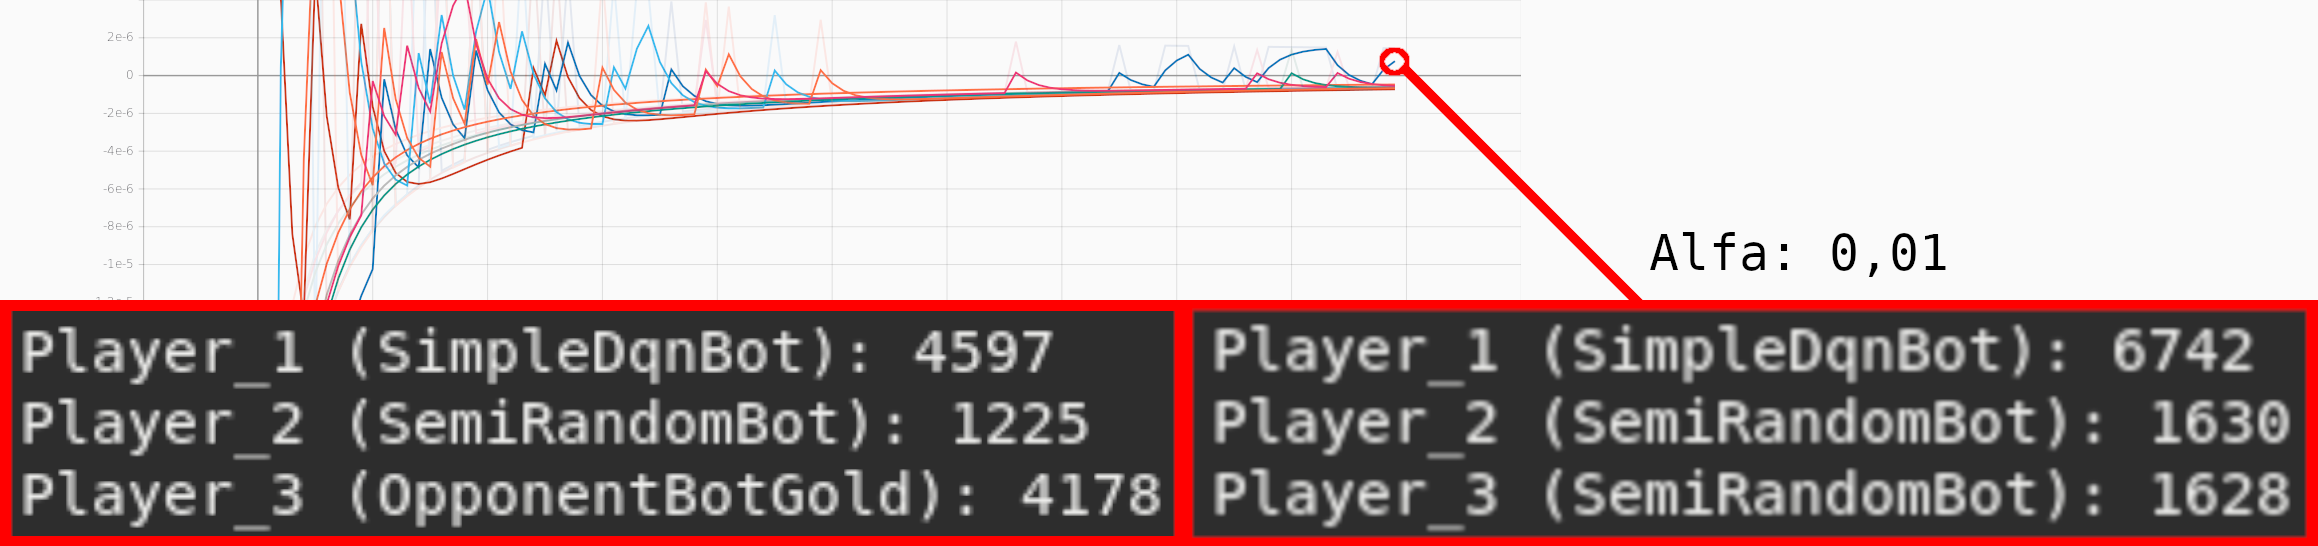
\includegraphics[width=0.8\linewidth,clip=]{images/final_model_result.png}%
	\figcaption{Rezultati konačne validacije}%
	\label{fig:final_model_result}%
\end{minipage}
\\[\intextsep]

Dodatni pokusi obuhvaćaju:
\begin{itemize}
	\item Neuronska mreža sa 3 skrivena sloja: Dodao se još jedan sloj neurona, za povećavanje neuronske mreže. Neuronska mreža se može povećati u širinu i u dubinu. U širinu znači povećavanje broja neurona u pojedinim skrivenim slojevima a u dubinu povećavanje broja skrivenih slojeva.
	\item Heuristično istraživanje: Umjesto nasumične odluke tokom istraživanja, heuristični agent donosi odluku. Agenta kroz trening vodi heuristični, što u jednu ruku ubrzaje trening ali u drugu ga ograničava.
	\item Zajednička neuronska mreža: Više agenata koriste istu neuronsku mrežu, tako da se mreža u jednoj epizodi više puta ažurira. 
\end{itemize}

Niti jedan od dodatnih pokusa nije donio znatno poboljšanje. Trening više agenata sa zajedničkom neuronskom mrežom se prekinuo, pošto se pojavio već poznati problem u kojemu mreža zaključi da najduže ostaje u igri kada stalno izvrši akciju \textit{fold}. Situacija pred samim krajem treninga je bila takva da svi igrači uvijek izvršavaju akciju \textit{fold}, prisilni ulozi su kružili od igrača do igrača i epizoda nije imala kraja.
